\begin{figure}[t]
\centering
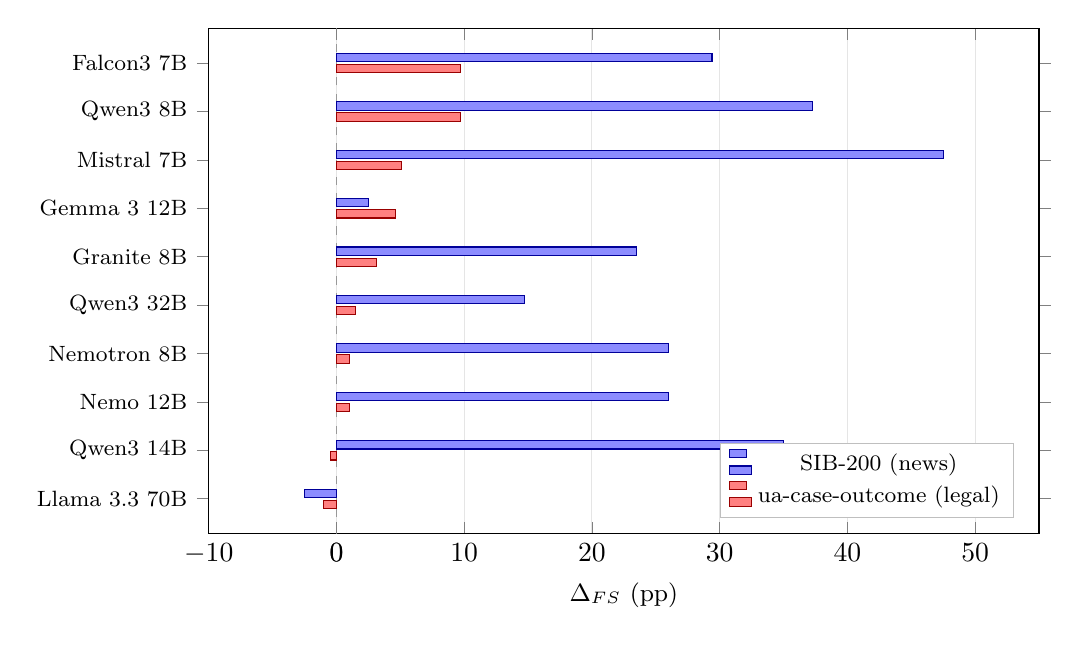
\begin{tikzpicture}
\begin{axis}[
    width=\columnwidth,
    height=8cm,
    xbar,
    bar width=3pt,
    xlabel={$\Delta_{\text{FS}}$ (pp)},
    symbolic y coords={
        {Llama 3.3 70B},
        {Qwen3 14B},
        {Nemo 12B},
        {Nemotron 8B},
        {Qwen3 32B},
        {Granite 8B},
        {Gemma 3 12B},
        {Mistral 7B},
        {Qwen3 8B},
        {Falcon3 7B}
    },
    ytick=data,
    yticklabel style={font=\footnotesize},
    xlabel style={font=\small},
    xmin=-10, xmax=55,
    legend style={
        at={(0.97,0.03)},
        anchor=south east,
        font=\footnotesize,
        draw=gray!50,
    },
    enlarge y limits=0.08,
    xmajorgrids=true,
    ymajorgrids=false,
    grid style={gray!20},
    extra x ticks={0},
    extra x tick style={
        grid=major,
        grid style={black!40, thin, dashed},
    },
]
\addplot[fill=blue!45!white, draw=blue!60!black, bar shift=2pt] coordinates {
    (-2.5,{Llama 3.3 70B})
    (35.0,{Qwen3 14B})
    (26.0,{Nemo 12B})
    (26.0,{Nemotron 8B})
    (14.7,{Qwen3 32B})
    (23.5,{Granite 8B})
    (2.5,{Gemma 3 12B})
    (47.5,{Mistral 7B})
    (37.3,{Qwen3 8B})
    (29.4,{Falcon3 7B})
};
\addplot[fill=red!50!white, draw=red!60!black, bar shift=-2pt] coordinates {
    (-1.0,{Llama 3.3 70B})
    (-0.5,{Qwen3 14B})
    (1.0,{Nemo 12B})
    (1.0,{Nemotron 8B})
    (1.5,{Qwen3 32B})
    (3.1,{Granite 8B})
    (4.6,{Gemma 3 12B})
    (5.1,{Mistral 7B})
    (9.7,{Qwen3 8B})
    (9.7,{Falcon3 7B})
};
\legend{SIB-200 (news), ua-case-outcome (legal)}
\end{axis}
\end{tikzpicture}
\caption{Few-shot effect by task and model. Every model that benefits on news benefits less on legal text; two models degrade on legal (below dashed line). Models sorted by legal $\Delta_{\text{FS}}$.}
\label{fig:task_contrast}
\end{figure}
